\ifdefined\included
\else
\setcounter{chapter}{5} %% Numéro du chapitre précédent ;)
\dominitoc
\faketableofcontents
\fi

\chapter{Estimating communication feasibility and cost at task planning}
\chaptermark{Estimating communication at task planning}
\minitoc

The contribution presented in this chapter is excerpted from our work, published in the proceedings of the ICSR 2020 conference~\cite{buisan_2020_human}. In this manuscript, the contribution is more detailed and discussed. In the continuity of the previous, the presented work has been achieved in collaboration with Guilhem Buisan. While his focus was on task planning, mine was on the link between the knowledge base as an ontology and the task planner. In this thesis, we will deepen this link and discuss possible improvements to the one initially presented.

\section{Introduction}

It is well established that a key aspect of the success of collaborative tasks is based on clear and fluent communication grounded in the context of the interaction. In the Natural Language Processing (NLP) research field and by extension in the Human-Robot Interaction (HRI) field, it has been divided into two dual problems~\cite{tellex_2020_robots}. On one hand, the Natural Language Understanding (NLU) aims the robot to interpret and grounds human's utterances with regard to the current situation and to react according to it~\cite{brawer_2018_situated}. In another hand, the Natural Language Generation (NLG) aims the robot to produce language. It could either be to ask for help~\cite{tellex_2014_asking}, to align knowledge~\cite{devin_2016_implemented}, or to explain its decision to its partner~\cite{roncone_2017_transparent}.

In the previous chapter, we have introduced an algorithm able to generate the content of a referring expression. Such contribution thus falls in the NLG problem. Considering the REG as an action that can be performed by the robot means that the robot could plan such communication in terms of \textbf{when} and \textbf{what} to communicate. While the "when" is directly handled by the task planner, the "what" is provided by the REG. However, the REG does not only provide the content but is also able to state if such communication is feasible or not and give information about its cost depending on the number of relations to communicate. Because the REG algorithm work on a knowledge base representing the current state of the environment, maintaining a comparable representation of the environment for the future states of the task (as it is done in symbolic task planning) would allow the robot to estimate the \textbf{feasibility} and the \textbf{cost} of the verbal communication actions all along with a task.

With these two pieces of information, a task planner could compare verbal communication with one another, compare with other means of communication, minimize the overall communication complexity, and prevent some plan failures. This approach to estimating the communication at task planning can be compared to the one proposed in~\cite{lallement_2016_symbolic}. In the latter, motion actions were evaluated at task planning to estimate their feasibility, costs, and indirect effects. With both approaches, the symbolic plans can be optimized and can be more reliable in preventing execution failures and thus the need for reparation.


\begin{figure}[t!]
\centering
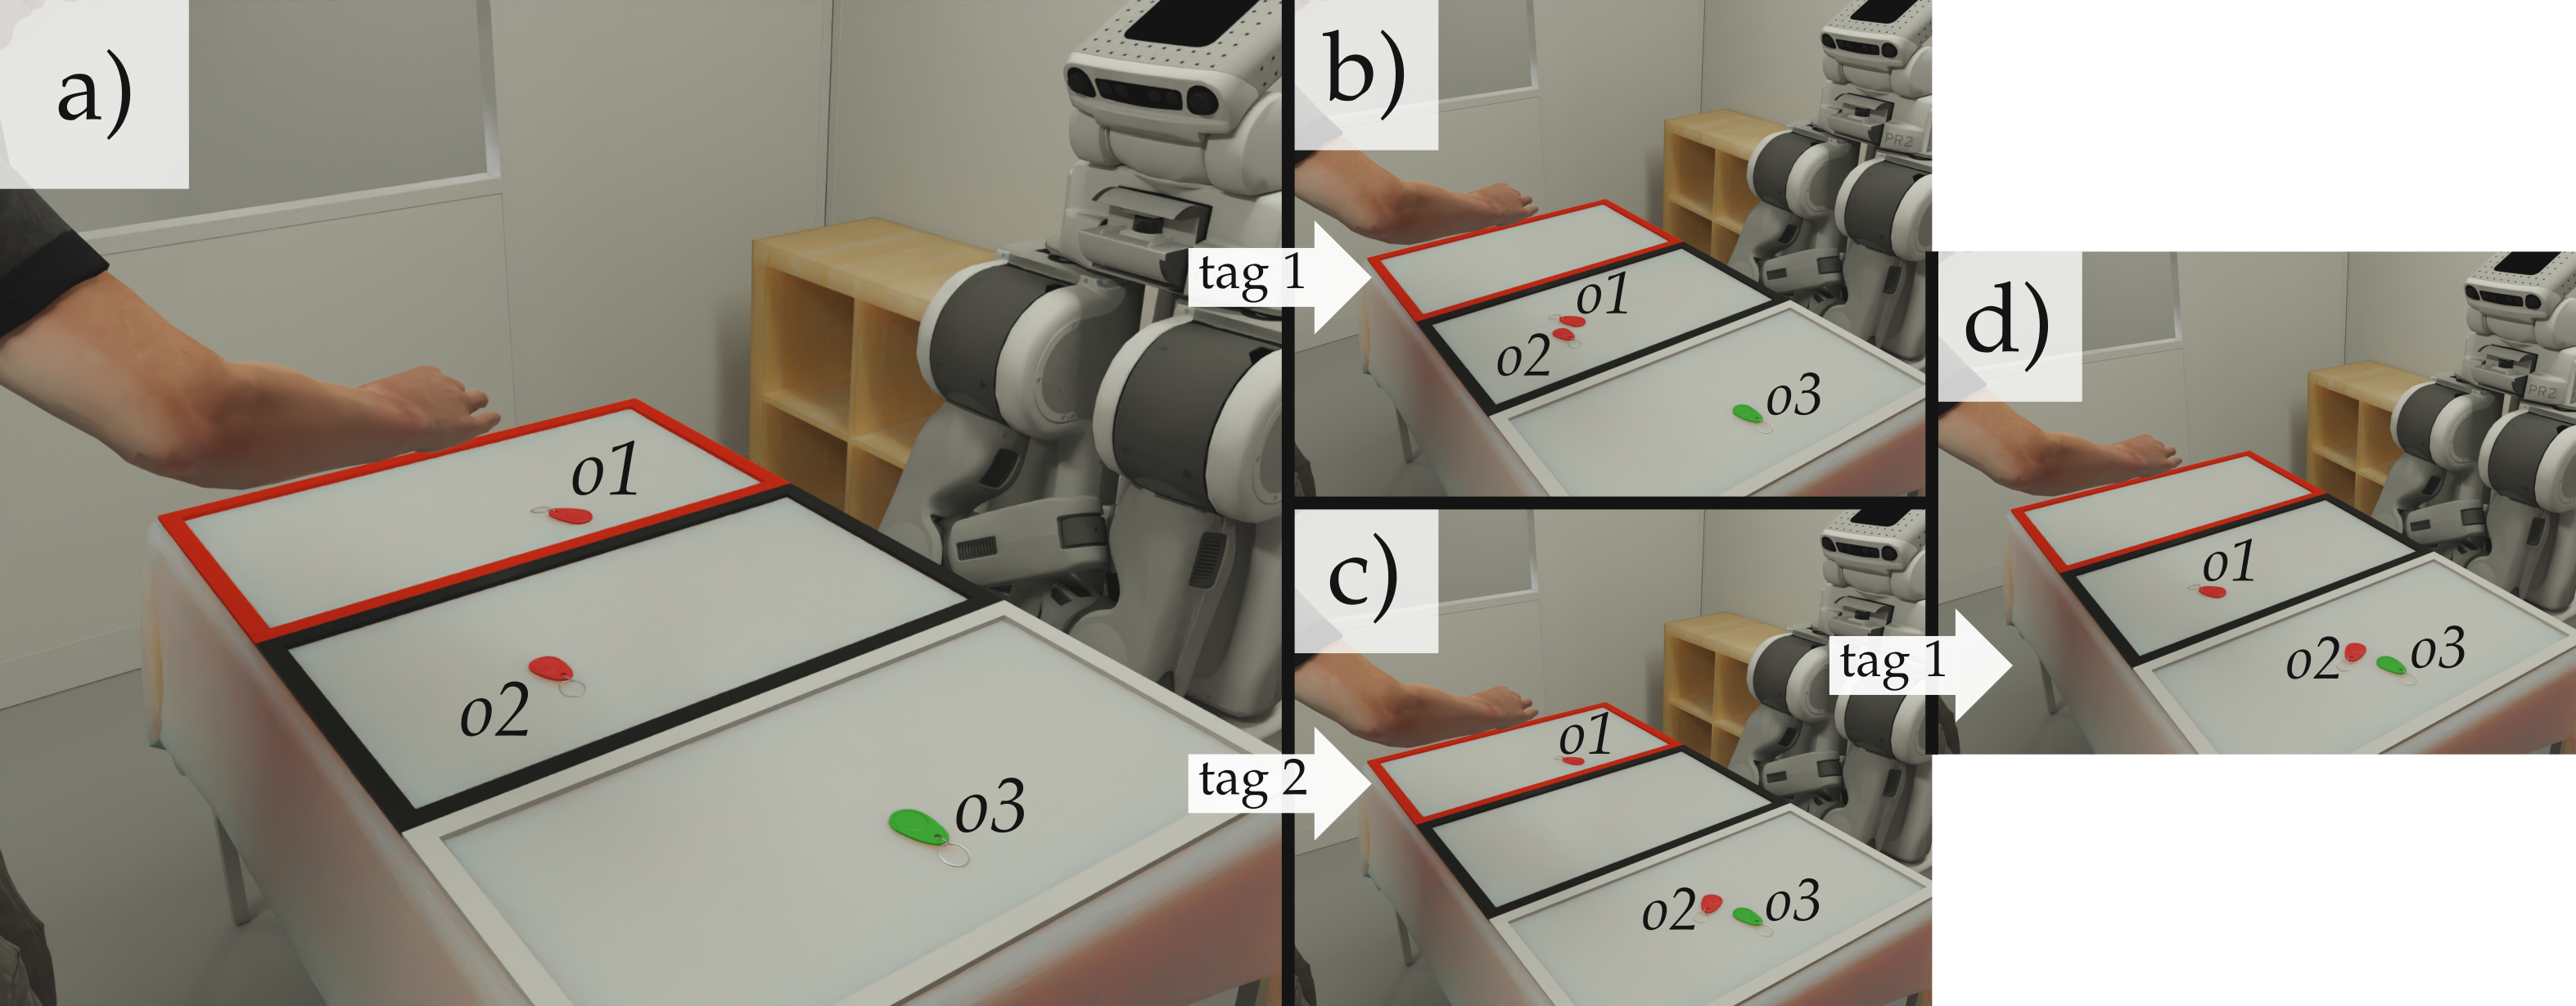
\includegraphics[width=\textwidth]{figures/chapter5/intro/intro.png}
\caption{\label{fig:chap5_intro} A Human-Robot collaborative task with three colored areas and three RFID tags (situation a). The robot has to explain to its human partner to put the tag \textit{o1} in the black area and the tag \textit{o2} in the white area, to reach the situation d. The objects identifiers' are only known to the robot.
If all the communications of the task are not planned ahead, a deadlocked situation could appear if the robot first asks to move the tag \textit{o1} before \textit{o2} (situation b).}
\end{figure}

%Consider the situation illustrated in Fig.~\ref{fig:introduction}. In this task the human and the robot have to put each cube in a specific colored area. The robot does not have the ability to act on the cubes and the human does not know the goal configuration. The robot must therefore communicate the successive actions that the human will have to perform. The two cubes are visually the same to the human, but the robot can identify them. The initial configuration is given in  Fig.~\ref{fig:introduction}a with the cube C1 in the red area and the cube C2 in the black area. The goal configuration (Fig.~\ref{fig:introduction}d) requires the cube C1 to be places in the black area and the cube C2 in the white area.
%In the case where the communication action is refined only at execution, a solution plan could be to tell the human to move the cube C1 in the black area then the cube C2 in the white one. The execution of this plan would result in: \textit{"Take the cube in the red area and put it in the black area"}. In this new situation where both cubes are now in the black area (Fig.~\ref{fig:introduction}b), the robot has no way to designate the cube C2 without ambiguity. Hence, the task is blocked.
%Taking into account the communication feasibility and cost estimation during the planning process would allow to find the solution where the robot tell to the human to move the cube C2 first (Fig.~\ref{fig:introduction}c) and then the cube C1 (Fig.~\ref{fig:introduction}d). Considering now that the robot can point to the cubes, the deadlock of the first solution can be avoided with a pointing action and nevertheless, thanks to the communication cost estimation, the least expensive solution can be selected.


%In \S\ref{sec:related_work}, we briefly discuss related work and how our contribution addresses new issues. Our approach and its components are then described in \S\ref{sec:Integration}. Three case studies are finally presented in \S\ref{sec:Case_studies} to show how this approach can be used to prevent deadlocked situations at execution, how it can reduce the global communication complexity during a Human-Robot collaborative task and how it can be used to balance between different communication means.

\section{Related work: The need to plan communication}


\section{The involved components}

\subsection{The Hierarchical Task Planner}

\subsection{The semantic knowledge base}

\subsection{The Referring Expression generator}


\section{Integrating task and communication planners}

\subsection{The representation os the communication action}

\subsection{Maintaining the right knowledge base, at the right time}


\section{Results}

\subsection{Prevent execution dead-end}

\subsection{Reduce the overall communication complexity}

\subsection{Compare with other communication means}